\documentclass[master=mai,masteroption=slt]{kulemt}
\setup{% Remove the "%" on the next line when using UTF-8 character encoding
  inputenc=utf8,
  title={Article-level Media Bias Classification},
  author={Stefan Liemawan Adji},
  promotor={Dr. Miryam de Lhoneux},
  assessor={},
  assistant={Dr. Timo Spinde and Tomáš Horych of Media Bias Group}
  }
% Remove the "%" on the next line for generating the cover page
%\setup{coverpageonly}
% Remove the "%" before the next "\setup" to generate only the first pages
% (e.g., if you are a Word user).
%\setup{frontpagesonly}

% Choose the main text font (e.g., Latin Modern)
\setup{font=lm}

% If you want to include other LaTeX packages, do it here. 

% Finally the hyperref package is used for pdf files.
% This can be commented out for printed versions.

\usepackage{hyperref}
\hypersetup{
    pdfusetitle,
    colorlinks,
    plainpages=false,
    citecolor=magenta,  
    linkcolor=black,  
    urlcolor=black,   
    filecolor=black   
}

\usepackage{verbatim}
\usepackage{tikz}
\usepackage{amsmath}
\usepackage{multirow}


\usepackage{algorithm}
\usepackage{algpseudocode}


%\includeonly{chap-n}
\begin{document}

% \begin{preface}
%     I would like to thank everybody who kept me busy the last year,
%     especially my promoter and my assistants. I would also like to thank the
%     jury for reading the text. My sincere gratitude also goes to my wive and
%     the rest of my family.
% \end{preface}

\tableofcontents*

\begin{abstract}
    In today's digital, information-rich society, media bias poses a significant challenge to the objectivity and credibility of news reporting. Media bias can shape our perceptions, influence our opinions, and affect our understanding on various issues. It is crucial to recognise and address this bias to ensure a well-informed and balanced perspective. By being aware of the inherent biases in media sources, individuals can critically evaluate the information they consume and seek out diverse viewpoints to form a more comprehensive understanding of the world. This thesis project aims to identify forms of media bias in articles and build a system to detect and classify media bias at the article level. The BAT \cite{spinde-2023-bat} dataset, containing articles annotated by Ad Fontes \cite{adfontes}, is extended by crawling article content from individual outlet websites. Using reliability scores as labels, the articles are categorised into four bias classes: Problematic, Questionable, Generally Reliable, and Reliable. Both the titles and content of the articles are used as primary features, with the influence of outlet metadata also examined. Several methods are proposed to tackle the task of article-level media bias classification using the extended BAT dataset. These methods include frequency-based approaches, BERT (sliding window) fine-tuning, and \textbf{BERT/MAGPIE CLS}: feature-based approach and CLS pooling continued with feeding into Transformer layers and Multi-Layer Perceptron (MLP).
\end{abstract}

% % A list of figures and tables is optional
% %\listoffigures
% %\listoftables
% % If you only have a few figures and tables you can use the following instead
% \listoffiguresandtables
% % The list of symbols is also optional.
% % This list must be created manually, e.g., as follows:
% \chapter{List of Abbreviations and Symbols}
% \section*{Abbreviations}
% \begin{flushleft}
%     \renewcommand{\arraystretch}{1.1}
%     \begin{tabularx}{\textwidth}{@{}p{12mm}X@{}}
%         LoG  & Laplacian-of-Gaussian      \\
%         MSE  & Mean Square error          \\
%         PSNR & Peak Signal-to-Noise ratio \\
%     \end{tabularx}
% \end{flushleft}
% \section*{Symbols}
% \begin{flushleft}
%     \renewcommand{\arraystretch}{1.1}
%     \begin{tabularx}{\textwidth}{@{}p{12mm}X@{}}
%         42    & ``The Answer to the Ultimate Question of Life, the Universe,
%         and Everything'' according to \cite{h2g2}                            \\
%         $c$   & Speed of light                                               \\
%         $E$   & Energy                                                       \\
%         $m$   & Mass                                                         \\
%         $\pi$ & The number pi                                                \\
%     \end{tabularx}
% \end{flushleft}

% Now comes the main text
\mainmatter

\chapter{Introduction}
\label{cha:1}

This thesis project is part of an Advanced Master of Artificial Intelligence programme—Speech and Language Technology, conducted in collaboration with the Media Bias Group \cite{media-bias-group}, who provided the topic and additional guidance along the project. The introduction chapter provides a general overview of the project, outlining its motivations, goals, and contributions.


\section{Motivation}

Media bias is widespread in today's landscape, particularly on matters such as health, climate, and politics \cite{suarez-2021-prevalence-health-misinformation,wang-2024-health-misinformation,fleming-2023-climate-disinformation,tiedemann-2024-misinformation-democracy}. The existence of media bias in news sources can and has been used as a way to shape and influence public opinion \cite{aires-2020-information}. The advent of social media has exacerbated the spread of misinformation, allowing false information to easily and rapidly circulate while remain unchecked \cite{froehlich-2024-misinformation}. A survey by \cite{allcott-2017-fake-news-election} indicated that fake news on social media played a significant role in the election of President Trump in 2016. During the COVID-19 pandemic, numerous conspiracy theories gained widespread traction through the media, with substantial support from large groups of people. A 2020 Harvard survey revealed that nearly 20\% of people believed the pandemic was a ploy "to install tracking devices inside our bodies" \cite{enders-2020-covid19-misinformation}. Despite being a major societal issue, research on the spread of misinformation on social media platforms remains scarce \cite{muhammed-2022-disaster-of-misinformation}.

\begin{figure}[htbp]
    \centering
    \fbox{
        \includegraphics[width=0.6\linewidth]{images/the-economist-biased-article.png}}
    \caption{A recent article from The Economist \cite{economist-2024-incels} portraying gender discrimination with a negatively framed headline}
    \label{fig:the-economist-biased-article}
\end{figure}

An example of a biased article can be seen in a recent piece published by The Economist \cite{economist-2024-incels}, shown in Figure \ref{fig:the-economist-biased-article}. The author presents the information in a way that could be considered biased due to its choice of language, implied causation, and lack of context. Published in June 2024, this example proves that media bias exists and is prevalent even in prominent news outlets like The Economist.

Ideally, unbiased media content that objectively and fairly represents multiple or a range of perspectives is desirable, news sources should remain neutral and let readers build their own opinions on the subject \cite{reuters-2021-digital-news-report}. However, this is often unachievable due to human capabilities and resource limitations; journalists cannot possibly possess complete knowledge on every topic, be physically present everywhere, or interview every relevant individual on a significant subject \cite{allsides-2022-bias-definition}. Truth and journalism objectivity is a complex matter full of choices and dilemmas, where ultimately it falls on the journalists' own preferences and criteria \cite{boudana-2011-journalistic-objectivity}. A survey found evidence that journalists' personal beliefs substantially influence their news decisions, expressed within the stories they choose and the statements they write \cite{patterson-donsbach-1996-news-decisions}.

Therefore, instead of eliminating media bias, our goal should be to draw attention to its existence and forms, giving readers awareness of such content \cite{spinde-2024-taxonomy}, ultimately building a tool to defend readers from media manipulation, political agenda or indoctrination. This is essential to ensure that readers are able to form their own choices and opinions with utmost honesty and transparency.

% Journalism has abandoned the idea of seeking neutrality and objectivity, aiming instead to adopt a more engaged and committed approach. Objectivity in the media has been rejected both as an impossible standard and as an undesirable norm. \cite{boudana-2011-journalistic-objectivity}.

While there exist organisations consisting of expert annotators that manually read and review articles \cite{adfontes, allsides, mbfc}, there is a growing need for more efficient methods of media bias detection. Automatic media bias detection offers a promising alternative, as developing robust systems could enhance scalability and consistency in identifying biases across a vast array of articles, addressing the limitations of manual review processes. However, this field remains relatively new, under-resourced, and challenging, due to the lack of a universally accepted definition of bias and its subtlety, which can make it difficult to identify \cite{rodrigo-2024-systematic-review-media-bias}.

Available media bias datasets \cite{spinde-2021-babe,fan-2019-basil,chen-2020-nlpcss,spinde-2023-bat,gruppi-2023-nela-gt-2022} are either limited in size or contain low-level, ambiguous annotations. In addition, these datasets vary in format, cover different sets of topics, contain different types of bias, and, more importantly, use different labelling formats, making it particularly difficult to compare and evaluate different media bias datasets and models trained on them. There is a critical need to develop new, richer datasets that are more extensive and varied, preferably covering a broader array of events and domains \cite{rodrigo-2024-systematic-review-media-bias}.

Existing works in media bias classification tend to have major drawbacks \cite{maab-2023-lexical-bias-detection, maab-2023-target-aware, guo-2022-modeling, van-den-berg-2020-context,lee-2021-unifying,lei-2022-sentence,lei-2024-event-relation}. The classification is mostly done on the sentence-level with binary output, which is far too naive and may miss the broader context and impact conveyed by an entire article. Sentence-level classifiers tend to also rely on low-level lexical information, which is proven to fail at the article-level \cite{chen-2020-detecting-media-bias-gaussian}. Moreover, different sentences within the same article can exhibit contradictory or varying biases \cite{lei-2022-sentence}. Thus, sentence-level classifiers are inadequate for accurately classifying media bias across an entire article. Since media content is typically presented as articles composed of numerous sentences, an effective article-level media bias classifier is both necessary and crucial.

While there are many studies focused on article-level political bias or ideology detection \cite{kulkarni-2018-multi-view,baly-2020-we-can-detect-your-bias,baly-2019-mt}, to my knowledge, there has been very little significant work on article-level media bias classification.

\section{Goals and Contributions}

The primary goal of this project is to develop a novel approach for article-level media bias classification, by considering State-of-the-Art (SOTA) transformer-based approaches, as well as techniques that have been proven to be successful in document classification \cite{su-2021-classifying,wan-2019-long-length,park-2022-efficient,pappagari-2019-hierarchical}. To achieve this, the project will address the following research questions:
\begin{enumerate}
    \item What are the challenges and limitations of article-level bias classification, and how can they be mitigated?
    \item How can current media bias datasets be improved to better support article-level classification?
    \item What are the most effective methods to represent articles and preserve contextual information for media bias classification task?
    \item How can an effective article-level media bias classifier be trained and evaluated?
\end{enumerate}

This thesis project makes three main contributions: (1) it investigates the current state of article-level media bias classification, identifying gaps in research and key challenges; (2) it reconstructs the BAT dataset by crawling articles content, resulting in a dataset of 5,497 articles with an additional multi-class labels; and (3) it examines various natural language processing (NLP) techniques for article-level media bias classification, highlighting that hierarchical methods show significant promise, slightly outperforming fine-tuning Longformer.

\section{About the Media Bias Group}

The Media Bias Group \cite{media-bias-group} was established in mid-2020 by Timo Spinde during his pursuit of a Ph.D. in computer science, having been integrated into the topic since his undergraduate studies, with a vision to aid others perceive news in a more balanced and conscious manner. After a year of planning how a system could uncover bias on a vast scale encompassing millions of articles, he founded the group and forged connections with various partners, particularly those relevant to specific aspects of the project. In just one year, the project has garnered support from multiple other research groups, with around twenty students from seven countries joining to contribute to the system. Since 2021, the group has also begun offering its first Ph.D. positions.

The group is comprised of a collective of scholars across various fields such as Psychology, Linguistics, and Computer Science, with a shared goal to comprehend the factors influencing human perception of news content as biased or one-sided. Currently, the network includes six main researchers and coordinators, twenty-one professors and postdocs, as well as eight active students. Numerous publications related to media bias have been published through the network into major conferences such as EMNLP 2021 \cite{spinde-2021-babe}, along with dataset and benchmark creations.


%%% Local Variables: 
%%% mode: latex
%%% TeX-master: "thesis"
%%% End: 
\chapter{Background Information and Literature Review}
\label{cha:2}


\section{Media Bias}

Allsides \cite{allsides-2022-bias-definition} defines media bias as "The tendency of news media to report in a way that reinforces a viewpoint, worldview, preference, political ideology, corporate or financial interests, moral framework, or policy inclination, instead of reporting in an objective way (simply describing the facts)". This phenomenon has existed and been researched since the 1950s \cite{white-1950-case-study-selection-news}, highlighting its enduring presence and impact on public perception. Media bias can manifest in various forms, including the selection of stories, framing of issues, and choice of language.

While biases may not always be intentional, they might cause significant consequences, possibly leading to inequalities and injustices. Some news outlets tend to use catchy headlines which trick readers into clicking, known as "clickbait", which are often ambiguous or misleading. Biased information can and has been used as a way to shape and influence public opinion \cite{aires-2020-information}. A survey of journalists from the United States, Great Britain, Germany, Italy, and Sweden found evidence that journalists' personal beliefs substantially influence their news decisions, expressed within the stories they choose and the statements they write \cite{patterson-donsbach-1996-news-decisions}.

\begin{figure}[htbp]
    \centering
    \fbox{
        \includegraphics[width=0.9\linewidth]{images/the-economist-biased-article.png}}
    \caption{A recent article from The Economist \cite{economist-2024-incels} portraying gender discrimination with a negative-framing headline}
    \label{fig:the-economist-biased-article}
\end{figure}

An example of a biased article can be seen from a recent article published by The Economist \cite{economist-2024-incels} in Figure \ref{fig:the-economist-biased-article}. The headline includes a negative framing of certain groups, which can influence readers' perceptions before they even read the article, suggesting that the existence of these groups is inherently problematic and harmful. Terms like "incels" (involuntary celibates) and "anti-feminists" carry strong negative connotations, which can evoke emotional responses and suggest a negative view of the groups mentioned. This is a strong example of framing bias.

\begin{figure}[htbp]
    \centering
    \includegraphics[width=0.9\linewidth]{images/bias-types-taxonomy.png}
    \caption{Media bias types as defined in the Media Bias Taxonomy \cite{spinde-2024-taxonomy}}
    \label{fig:bias-types-taxonomy}
\end{figure}

Media bias can manifest within different levels, categorised into 4 major types \cite{spinde-2024-taxonomy}, as shown in Figure \ref{fig:bias-types-taxonomy}. This project will mainly focus to address text-level context bias: phrasing bias, spin bias, and statement bias \cite{spinde-2024-taxonomy}: statement bias occurs when media personnel insert their personal views into the content, phrasing bias is marked by the use of provocative or non-neutral language, spin bias is introduced when essential information is omitted from the narrative.

Another particularly dangerous example of media bias is its application in relation to elections. According to a survey done by \cite{allcott-2017-socialmedia-2016election}, fake news propagated in social media played a pivotal role in the eventual election of President Trump during the 2016 election. Panagopoulos' study \cite{panagopoulos-2020} revealed systemic biases leaning towards Democratic candidates during national and state levels pre-election polls conducted during the 2020 U.S. general election cycle. Rafail et al. \cite{rafail-2018-tea-party} examined 201,678 media documents from Tea Party organizations, Fox News, MSNBC, and 785 newspapers, revealing significant differences in how the Tea Party frames itself compared to how other media sources frame the movement, MSNBC portrays it as the worst aspect of the Republican Party, while Fox News sees it as the best, sharply in contrasts with how activists frame the movement as conservative but not strictly Republican, often clashing with Republican Party goals.

\begin{comment}
An analysis by Pew Research Center \cite{pew-2021-election2020} found that miscalculations observed in the 2020 U.S. election polls would adjust public opinion on issues by an average of just under 1 percentage point. Although errors of such scale would not have produced substantial differences on the American public opinions, this shows the underlying bias within polls specifically and the failure of accurately representing surveys.
\end{comment}

The phenomenon of media bias in media has not gone unnoticed, particularly by readers and consumers, lowering public trust in media outlets. In the United States particularly, trust in news media is at an all time low, falling consistently and significantly over the past 20 years \cite{pew-2021-partisan-divides, gallup-knight-2020-american-views, reuters-2023-digital-news-report}. Approximately half of Americans believe that the media is significantly responsible for the political divisions within the United States, with a growing number of Americans losing faith in the media's objectivity and perceiving it as actively engaging in ideological wars \cite{gallup-knight-2020-american-views}. Reuters Institute reported only less than half of their respondents (40\%) generally trust the majority of news sources, with the US ranked on 29 out of 40 countries (32\%) \cite{reuters-2023-digital-news-report,reuters-2023-trust}, ranking far below other countries such as Indonesia, Phillipines, and Turkey (full figure shown in Figure \ref{fig:trustworthiness-of-news-media-worldwide-2023}).

Readers themselves are not exempt from bias, as they are known to prefer to pick, follow, and consume articles that align with their own beliefs and ideology, an issue known as filter bubble \cite{lim-2018-understanding} or selective exposure \cite{spinde-2024-taxonomy}. This incident reinforces existing biases and limits exposure to diverse perspectives, creating echo chambers that hinder critical thinking and informed decision-making. The combination of media bias and filter bubbles can distort reality, perpetuate misinformation, and deepen societal divisions.


\begin{figure}[htbp]
    \centering
    \includegraphics[width=0.9\linewidth]{images/statistic_id1317019_consumers-witnessing-false-information-on-certain-topics-worldwide-2023.png}
    \caption{The rate of news consumers witnessing false or misleading information on several recent key topics in February 2023 \cite{reuters-2023-false-info}}
    \label{fig:consumers-witnessing-false-information-on-certain-topics-worldwide-2023}
\end{figure}


\begin{figure}[htbp]
    \centering
    \includegraphics[width=0.9\linewidth]{images/statistic_id1462057_frequency-of-seeing-false-information-online-in-the-us-2023-by-age-group.png}
    \caption{Frequency of seeing false or misleading information online in the United States as of April 2023, by age group \cite{yougov-2023-frequency}}
    \label{fig:frequency-of-seeing-false-information-online-in-the-us-2023-by-age-group}
\end{figure}

Based on surveys from Reuters and YouGov (shown in Figure \ref{fig:consumers-witnessing-false-information-on-certain-topics-worldwide-2023} and Figure \ref{fig:frequency-of-seeing-false-information-online-in-the-us-2023-by-age-group}), the United States is shown to have the highest rate in politics, COVID-19, and climate change, with nearly half of the respondents claimed to have seen false or misleading information in the last week. Furthermore, most adults of every age group responded to seeing false or misleading information on a \textbf{daily} basis. These numbers are deeply concerning, highlighting the extent of the misinformation and media bias problem in the US.

Ideally, unbiased media content that objectively and fairly represents multiple or a range of perspectives is desirable, news sources should remain neutral and let readers build their own opinions on the subject \cite{reuters-2021-digital-news-report}. However, this is often unachievable due to human capabilities and resource limitations; journalists cannot possibly possess complete knowledge on every topic, be physically present everywhere, or interview every relevant individual on a significant subject \cite{allsides-2022-bias-definition}. Truth and journalism objectivity is a complex matter full of choices and dilemmas, where ultimately it falls on the journalists' own preferences and criteria \cite{boudana-2011-journalistic-objectivity}.

Therefore, instead of eliminating media bias, our goal should be to draw attention to its existence and forms, giving readers awareness of such content \cite{spinde-2024-taxonomy}, ultimately building a tool to defend readers from media manipulation, political agenda or indoctrination. This is essential to ensure that readers are able to form their own choices and opinions with utmost honesty and transparency.


\section{Word Embeddings}

\begin{figure}[htbp]
    \centering
    \includegraphics[width=0.9\linewidth]{images/word_embeddings.png}
    \caption{Word embeddings visualisation \cite{narayanan-2019-word-embeddings}}
    \label{fig:word-embeddings}
\end{figure}

Word embeddings are a way to represent words in a continuous vector space where words with similar meanings are placed close to each other, thereby capturing semantic relationships between words. This approach gained significant popularity with the introduction of \textit{word2vec} as a method to generate word embeddings \cite{mikolov-2013-embeddings}. Most Natural Language Processing (NLP) tasks approaches still inherently rely on word embeddings to represent textual data, often serving as the initial input to models. An example of word embeddings is visualised in Figure \ref{fig:word-embeddings}.


\section{MultiLayer Perceptron (MLP)}

\begin{figure}[htbp]
    \centering
    \includegraphics[width=0.9\linewidth]{images/mlp.png}
    \caption{MultiLayer Perceptron visualisation \cite{perez-enciso-2019-guide}}
    \label{fig:mlp}
\end{figure}

A MultiLayer Perceptron (MLP) is a fully connected Artificial Neural Network (ANN) that consists of single or multiple hidden layers, illustrated in Figure \ref{fig:mlp}. Hidden layers refer to the collection of neurons that are between the input and output layers, transforming data from layer to layer \cite{uzair-2020-hidden-layers}. The weighted sum (\( \mathbf{z} \)) in a hidden layer of a neural network is computed as follows (Equation \eqref{eq:z}):

\begin{equation}
    \label{eq:z}
    \mathbf{z} = \mathbf{W}\mathbf{x} + \mathbf{b}
\end{equation} where \( \mathbf{x} \) is the input vector, \( \mathbf{W} \) is the weight matrix, \( \mathbf{b} \) is the bias vector. After computing \( \mathbf{z} \), an activation function \( f \) is applied element-wise to produce the output \( \mathbf{h} \) (Equation \eqref{eq:h}):

\begin{equation}
    \label{eq:h}
    \mathbf{h} = f(\mathbf{z})
\end{equation}

MLP is widely used due to its ability to introduce non-linearity into the model, allowing the network to approximate complex functions that are beyond the capability of simple linear models. By integrating multiple hidden layers with non-linear activation functions, MLP can learn intricate patterns and relationships within data, making them suitable for a wide range of machine learning tasks. This flexibility is pivotal in capturing the nuanced and intricate structures inherent in real-world datasets, thereby enhancing the model's predictive accuracy and generalisation capabilities.


\section{Long Short-Term Memory (LSTM)}

\begin{figure}[htbp]
    \centering
    \includegraphics[width=0.9\linewidth]{images/lstm.jpeg}
    \caption{LSTM architecture \cite{rahman-2023-lstm-networks}}
    \label{fig:lstm}
\end{figure}

LSTM \cite{hochreiter-1997-lstm} is a type of Recurrent Neural Network (RNN) architecture designed to address the vanishing gradient problem and capture long-term dependencies in sequential data. It incorporates two fundamental components: memory cells and gates. Memory cells maintain a cell state, which can store information over long sequences and allows the model to retain information for longer durations compared to traditional RNNs. Gates control the flow of information into and out of the memory cell, controlled by sigmoid and tanh activation functions, which regulate the information flow based on the input data and the current state. Figure \ref{fig:lstm} shows the full architecture of a LSTM block.


\section{Transformer and Large Language Model (LLM)}

\begin{figure}[htbp]
    \centering
    \includegraphics[width=0.7\linewidth]{images/transformer.png}
    \caption{Transformer visualisation \cite{vaswani-2023-attention}}
    \label{fig:transformer}
\end{figure}

The Transformer architecture relies entirely on attention mechanism to capture global dependencies across input and output sequences, allowing for unprecedented levels of parallelisation instead of sequential processing \cite{vaswani-2023-attention}. Their introduction marks a fundamental shift away from traditional sequence-based models like recurrent neural networks (RNNs) and convolutional neural networks (CNNs), offering unparalleled advancements in handling long-range dependencies and contextual information. Their effectiveness stems from the attention mechanism, specifically through self-attention and multi-head attention mechanisms, defined in Equation \eqref{eq:attention} and \eqref{eq:multihead} \cite{vaswani-2023-attention}. These mechanisms allow the network to weigh and prioritise relevant information across sequences, capturing intricate relationships and semantic nuances.

LLMs are artificial neural networks that utilise the transformer architecture, designed to understand and generate human language. They are trained on vast amounts of diverse text data using unsupervised learning techniques, often containing millions or even billions of parameters. Two of the most popular and widely used LLMs are \textbf{Bidirectional Encoder Representations from Transformers (BERT)} \cite{devlin-2019-bert}, comprised of 110 million parameters, and GPT, particularly GPT-4 \cite{openai-2024-gpt4}, which is reported to have an astonishing 1.76 trillion parameters, based on a report by SemiAnalysis in 2023 \cite{semianalysis-gpt4}.

\textbf{Fine-tuning} is a way to optimise pre-trained LLMs to for specific tasks or domains, aiming to achieve improved inference quality with limited resources. \cite{oracle-finetuning-blog}. During this process, the model weights are adjusted based on the training data for the downstream task, allowing the model to adapt its pre-trained representations to the specific requirements of the task. This approach leverages the powerful pre-trained representations from LLMs and adapts them with relatively small amounts of task-specific training data. It has become a widely common and popular technique for performing various NLP tasks due to its effectiveness in improving performance over traditional models.

\begin{figure}[htbp]
    \centering
    \includegraphics[width=0.9\linewidth]{images/bert_finetuning.png}
    \caption{BERT pre-training and fine-tuning procedures \cite{devlin-2019-bert}}
    \label{fig:bert_finetuning}
\end{figure}

\begin{equation}
    \label{eq:attention}
    \text{Attention}(\mathbf{Q}, \mathbf{K}, \mathbf{V}) = \text{softmax}\left( \frac{\mathbf{Q}\mathbf{K}^\top}{\sqrt{d_k}} \right) \mathbf{V}
\end{equation}

\begin{equation}
    \label{eq:multihead}
    \text{MultiHead}(\mathbf{Q}, \mathbf{K}, \mathbf{V}) = \text{Concat}(\text{head}_1, \ldots, \text{head}_h) \mathbf{W}^O
\end{equation}
where
\[
    \text{head}_i = \text{Attention}(\mathbf{Q} \mathbf{W}^Q_i, \mathbf{K} \mathbf{W}^K_i, \mathbf{V} \mathbf{W}^V_i)
\]

Transformers and LLMs have sparked a revolution in the domain of Artificial Intelligence (AI), having achieved remarkable successes across diverse fields such as natural language processing, computer vision, and audio processing \cite{lin-2022-survey-transformers}. They have single-handedly catalysed the emergence of a new era in AI capabilities observed today, predicted to have an even greater influence than the Industrial and digital revolutions combined \cite{makridakis-2017-ai-revolution}.

\section{MAGPIE}

\begin{figure}[htbp]
    \centering
    \includegraphics[width=0.9\linewidth]{images/magpie.png}
    \caption{MAGPIE containing a pre-trained representation of various biases \cite{horych-2024-magpie}.}
    \label{fig:magpie}
\end{figure}

\textbf{MAGPIE} \cite{horych-2024-magpie} is a large-scale, RoBERTa-based, multitask pre-training approach specifically designed for media bias detection, pre-fine-tuned on fifty-nine bias-related tasks covering a broad spectrum of biases. Pre-fine-tuning is a large-scale training phase situated between language model pre-training and fine-tuning. It involves extensive multitask learning (MTL) and aims to foster the development of representations that generalise more effectively across various tasks \cite{aghajanyan-2021-muppet}. Pre-fine-tuning allows multitask-approach such as MAGPIE to generalise better on various tasks related to media bias, enabling better performance on these tasks compared to single-task RoBERTa approach \cite{horych-2024-magpie}.

Unfortunately, MAGPIE is only trained to output binary classification (biased or unbiased) and mostly trained on sentences, therefore unable to be fine-tuned for article-level media bias classification task. However, the model and its feature representations can still be utilised for a feature-based approach \cite{sun-2020-fine-tune}.


\section{Chunking and Hierarchical Techniques}

\begin{figure}[htbp]
    \centering
    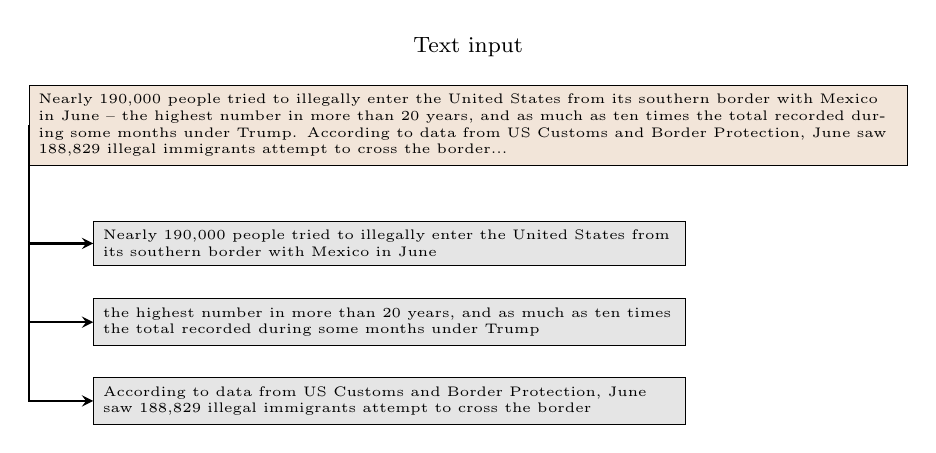
\begin{tikzpicture}
        \tikzstyle{arrow} = [thick,->,>=stealth]
        \tikzstyle{chunk} = [rectangle, draw, fill=gray!20, font=\tiny, text width=0.6\linewidth, align=left]
        \tikzstyle{label} = [text centered,font=\footnotesize]

        \node[label] at (0, 1) {Text input};
        \node (input) [draw, align=left, text width=0.9\linewidth, font=\tiny, fill=brown!20] at (0, 0) {Nearly 190,000 people tried to illegally enter the United States from its southern border with Mexico in June – the highest number in more than 20 years, and as much as ten times the total recorded during some months under Trump. According to data from US Customs and Border Protection, June saw 188,829 illegal immigrants attempt to cross the border...};

        \node[chunk] (chunk1) [draw] at (-1, -1.5) {Nearly 190,000 people tried to illegally enter the United States from its southern border with Mexico in June};
        \node[chunk] (chunk2) [draw] at (-1, -2.5) {the highest number in more than 20 years, and as much as ten times the total recorded during some months under Trump};
        \node[chunk] (chunk3) [draw] at (-1, -3.5) {According to data from US Customs and Border Protection, June saw 188,829 illegal immigrants attempt to cross the border};

        \draw[arrow] (input.west) |- (chunk1.west);
        \draw[arrow] (input.west) |- (chunk2.west);
        \draw[arrow] (input.west) |- (chunk3.west);
    \end{tikzpicture}
    \caption{Illustration of chunking}
    \label{fig:chunking}
\end{figure}


\textbf{Chunking} is a technique used to break down text into smaller, more manageable units. This technique can be applied to segment documents into smaller paragraphs or sentences, as illustrated in Figure \ref{fig:chunking}, facilitating more efficient processing and analysis. \textbf{Hierarchical models} incorporate multiple levels of abstraction or granularity to capture complex relationships within data. These models are particularly useful when dealing with structured data that naturally falls into a hierarchical organisation, such as documents composed of paragraphs and sentences. Furthermore, \textbf{hierarchical transformer model} is a variant of the transformer architecture that incorporate hierarchical structures to handle long sequences more efficiently. These models process data at different levels, such as sentences within paragraphs, to capture hierarchical relationships. Figure \ref{fig:hi_transformer} shows an example of hierarchical transformer modelused to produce document embeddings by utilising sentence-level and word-level information \cite{wu-2021-hi-transformer}.

\begin{figure}[htbp]
    \centering
    \includegraphics[width=0.9\linewidth]{images/hi_transformer.png}
    \caption{An example of hierarchical transformer model, Hi-Transformer\cite{wu-2021-hi-transformer}, to model long document}
    \label{fig:hi_transformer}
\end{figure}

\section{Document Classification}

Automatic document classification is first mentioned in 1963 \cite{borko-1963-auto-doc-classification}, with earlier text processing concepts and techniques defined in the 1950s \cite{luhn-1958-business-intelligence-system}. Document classification refers to the task of classifying text documents, commonly include large text processing and handling with various structure and content type. Typical use cases may include work with legal and financial documents, reports, and managing digital libraries.

In 2022, according to International Data Corporation (IDC) report, unstructured data accounted for 90\& of the total of organisation-generated data, in forms of purchase orders, product inventories, import/export records, sales agreements, contracts, patents, patient treatment notes, financial earning reports, and employee performance records, among many others \cite{box-2023-untapped}. Unstructured data refers to unorganised data that cannot be stored well into database, commonly in form of large collections of texts, terabytes or petabytes in size and growing exponentially \cite{mishra-2017-structured-unstructured}. Thus, the need to automatically manage and organise large amount of text and retrieve useful knowledge (knowledge discovery) is highly apparent \cite{mali-2021-relevance-of-preprocessing}.

Automatic document classification is an active area of research, with a primary focus on methods capable of handling long sequences and extracting relevant knowledge or information. Convolutional Neural Networks (CNN) \cite{afzal-deepdocclassifier,liu-2017-xmlcnn} and Hierarchical Attention Networks (HAN) \cite{yang-2016-han} have been traditionally used for this task. However, these approaches were later outperformed by DocBERT \cite{adhikari-2019-docbert}, which achieved superior results by leveraging knowledge distillation from the BERT-large model.

Straightforward, fine-tuning an encoder-based language model such as BERT is not necessarily effective for document-level processing as they are only able to process a maximum of 512 tokens, prompting significant information loss. Moreover, classification models that demonstrated significant results have been shown to perform poorly or even fail when they are tested on large documents \cite{wan-2019-long-length}.

There exist other LLMs that are designed specifically to handle longer sequences: Longformer \cite{beltagy-2020-longformer}, BigBird \cite{zaheer-2021-bigbird}. Both are hierarchical transformer models that utilises combination of global and local attention mechanisms. However, Longformer has been reported to not consistently surpass the baseline models in classification of long documents, performing only notably better than the baseline models on only two datasets \cite{park-2022-efficient}.

Several techniques have been implemented to combat the problem of handling long sequences, namely chunking and hierarchical techniques, as described previously. Pappagari et al. \cite{pappagari-2019-hierarchical} are among the first to utilise the transformer architecture for long sequences classification, introducing chunking and propagation methods. Su et al. \cite{su-2021-classifying} used chunking methods in a hierarchical transformer model with 'CLS-Pooling' (as also described in \cite{adhikari-2019-docbert}) to extract representations on the document-level for the task of clinical document classification. Khandve et al. \cite{khandve-2022-hierarchical-longdoc} also implemented a hierarchical model by utilising BERT and Bi-LSTM layers for long document classification tasks.


\section{Article-Level Media Bias Classification}

Article-level classification can be seen as a subset of document classification that specifically targets articles. This field focuses on categorising article-like texts such as news pieces, blogs, and other similar formats that typically comprise multiple paragraphs. Article-level media bias classification refers to the task of detecting and classifying media bias contained within a text. Article contents length generally falls between medium to long sequences, as they are not as lengthy as legal documents or clinical studies that typically contain multiple pages of text. Most news articles stay between several hundred to several thousand words.

Current available datasets for article-level and media bias classification in general are quite limited, often varying in formats or covering different types of bias. The \textbf{BASIL} dataset \cite{fan-2019-basil} is the most commonly used bias dataset, containing 300 articles with both article-level and phrase-level annotations. This dataset focuses on informational bias in news articles as it appears more frequently than lexical bias. However, the obvious drawback of this dataset is the low amount of articles included as it is not nearly enough data to get a good working detection model. \textbf{NLPCSS} \cite{chen-2020-nlpcss} (6964 articles), annotated via Ad Fontes labels, contains article-level textual content with three bias labels (bias, neutral, or unknown). Focusing on political bias and unfairness, this dataset can potentially serve as a suitable resource for an article-level media bias classification task. The \textbf{BAT} \cite{spinde-2023-bat} dataset (6345 articles, 321 outlets, Ad Fontes labels) is the most suitable for article-level bias detection as it supplies both bias-score and reliability-score for the whole article. However, the dataset itself does not supply the textual content of the articles and therefore needs to be extended, something that I have been working on as well during my Master's Thesis this and last year.

Furthermore, annotating media bias is not a straightforward task. Traditionally, this is done by hiring experts and journalists to manually read and determine how biased the content is. Here it is important to use multiple annotators to minimise introducing another form of bias towards the dataset. This comes with its own set of challenges as annotators might not always agree on biased text \cite{lim-2018-understanding}. As with \cite{spinde-2021-babe}, annotations are generally compiled and majority voted to achieve the final annotation given a particular text. Moreover, annotators' personal background moderately influenced their decisions and should be taken into consideration when building datasets, along with other factors such as topics, reading news habits, and honest mistakes \cite{spinde-2021-bias-words}. Clearly, this is not a cheap procedure and can act as a bottleneck when building a reliable media bias dataset.

Alternatively, organisations such as Allsides \cite{allsides} and Ad Fontes \cite{adfontes} have their own experts and annotations which can be crawled and exploited. Several papers and datasets \cite{spinde-2023-bat,chen-2020-nlpcss,kulkarni-2018-multi-view} have utilised this approach. However, since these datasets depend on manual labeling from third-party organisations, the selection of articles likely also introduces bias into the dataset \cite{spinde-2023-bat}.

Current State-of-the-Art (SOTA) approaches in media bias classification typically employs a transformer-based approach, either by fine-tuning or exploiting Large Language Models such as BERT \cite{devlin-2019-bert} or RoBERTa \cite{liu-2019-roberta}.

Past works on media bias classification typically use the BASIL dataset, operating on a sentence-level and outputting binary result (either biased or not) \cite{maab-2023-lexical-bias-detection, maab-2023-target-aware, guo-2022-modeling, van-den-berg-2020-context,lee-2021-unifying,lei-2022-sentence,lei-2024-event-relation}, complemented by the lack of appropriate and adequate datasets with article-level annotations \cite{demidov-2023-political-bias-classification}. Hence, \textbf{There are only a few existing studies on article-level media bias classification}. Chen et al. \cite{chen-2020-detecting-media-bias-gaussian} utilised a Gaussian mixture model, incorporating probability distributions of frequency, positions, and sequential order of lexical and informational sentence-level bias to detect article-level bias. Kulkarni et al. \cite{kulkarni-2018-multi-view} proposed a more complex model that leverages signals from multiple views to predict the political ideology of news articles, demonstrating that incorporating cues from the title, link structure, and content surpasses the state-of-the-art performance significantly. Given that automated text classification of news articles has been shown to benefit from using article segments instead of sentences as units of analysis, with preferences on supervised machine learning techniques \cite{barbera-2021-article-classification}, it may be advantageous to consider segment-length window size when developing methodologies.


%%% Local Variables: 
%%% mode: latex
%%% TeX-master: "thesis"
%%% End: 
\chapter{Dataset Reconstruction}
\label{cha:3}

\section{BAT dataset} \label{bat-characteristics}

The BAT dataset \cite{spinde-2023-bat} is selected for this project due to its suitability for article-level analysis (contains titles, URLs of articles, and outlet information) and better labelled with reliability score instead of binary label or political alignment (left, right). The dataset contains 6345 rows of manually labelled news articles from 255 English-speaking news outlets (US-based), originally scraped from Ad Fontes Media's website along with their respective \textbf{political bias} and \textbf{reliability scores}. Articles in the dataset encompassed a wide range of topics such as COVID-19, politics, and lifestyle. The political bias score measures the extent of political influence, ranging from -42 (most extreme left) to +42 (most extreme right). The reliability score reflects the article's truthfulness, with values ranging from 0 (least reliable, containing inaccurate or fabricated information) to 64 (most reliable, original fact reporting).

Both political bias and reliability scores on each article were rated using defined metrics and multiple sub-factors. Each article is rated by a politically balanced panel (right-leaning, centre, and left-leaning) of at least three analysts, selected from Ad Fontes Media's team of over 60 experts. Scores are then compared, discrepancies discussed and adjusted if necessary, before averaging for the final rating \cite{adfontes-methodology}. The reliability score evaluates original fact reporting to analysis, opinion, propaganda, and inaccurate/fabricated information, with scores above 40 generally considered good and scores below 24 typically seen as problematic, scores between 24 and 40 suggest a variety of factors, including a strong presence of opinion and analysis or significant variability in reliability across different articles \cite{adfontes-bias-reliability}. No further information can be found regarding the specific values and range of these rating, it can be safely assumed that this is an inherent part of their algorithms and methodology. Nevertheless, reliability score is chosen as the main label in this project due to its correlation with textual-level bias: phrasing bias, spin bias, and statement bias as described in Chapter \ref{cha:2}.

\begin{figure}[htbp]
    \centering
    \begin{minipage}{0.9\linewidth}
        \begin{center}
            \small{Trump Win Validated by Quantum Blockchain System Recount of Votes}
        \end{center}
        \scriptsize{
            A recount of voting ballots nationwide was being done by elite units of the National Guard by early Sun. morning 8 Nov. To prevent fraud official ballots had been printed with an invisible, unbreakable code watermark and registered on a Quantum Blockchain System. As of this writing, in five states 14 million ballots had been put through a laser scanner – 78\% of which failed because there was no watermark to verify the ballot. Of those that failed 100\% had checked for Biden. An initial test showed that according to water marks on validated ballots fed into the Quantum Computer, Trump won re-election by over 80\% of the legal ballot cast. The final validated vote tallied in that test: Trump 73.5 million votes to Biden’s 25.9 million – and that didn’t even account for Trump votes that people observed being tossed and never accounted for. Interesting enough, those figures corresponded with the two men’s Twitter accounts: Trump had 88.8 million followers to Biden’s 16.6 million. Using ‘infrared’ equipment that read which ballots were real, or fake the elite National Guardsmen had been deployed to the twelve targeted states of Alabama, Arizona, Pennsylvania, Colorado, Texas, Wisconsin, Tennessee, Washington, Virginia, Delaware, Illinois and Kentucky. In all nationwide, over 500 National Guardsmen were on guard over all ballot counting units. There was much more to the tests for fraudulent voting. In addition to the watermark these official ballots also contained ink made of corn, which created an electronic radiation circuit ID that could trace the location of that ballot through GPS transmission. In other words, they could trace if the ballot was filled out by the person named on the ballot. The Trump team would be filing a number of lawsuits onThey had been preparing for this for a long time under an election fraud investigation called Project Veritas. Judicial Watch:“Our new study shows 1.8M excess, or ‘ghost’ voters in 353 counties across 29 states. The data highlights the recklessness of mailing blindly ballots/ballot applications to voter registration lists,”@TomFitton Watch more: at http://judicialwatch.org Pennsylvania alone Trump’s legal counsel Rudy Guliani had testimony of 50-60 poll watchers who claimed being deprived of an ability to inspect mail in ballots. Nationally, noted attorney Sydney Powell (rumored to be appointed the next FBI director) said, “Hammer and Scorecard – the NSA Security Software turned illegal Election Software – ran an algorithm that gave Biden a 3\% vote advantage in Wisconsin, Michigan, Pennsylvania, Georgia, Nevada and Arizona.”Rest assured, all legal issues would be accounted for by the time the Electoral College met on. By then real election results – post court battles – would determine all legally cast ballots. The joint session of Congress would make the election official on 3 Jan. 2021.}
    \end{minipage}
    \caption{Example of a biased article, reliability score: 4.67}
    \label{fig:example-biased-article-1}
\end{figure}

An example of a low-rated article can be seen in Figure \ref{fig:example-biased-article-1}. The deceptive article contains many wrongful claims and blatantly fabricated events. In contrast, Figure \ref{fig:example-nonbiased-article-1} shows an example of a high-rated article. The content reports only facts regarding the event and statements from people related to the incident. Journalist opinions or political innuendos are non-existent.


\begin{figure}[htbp]
    \centering
    \begin{minipage}{0.9\linewidth}
        \begin{center}
            \small{Trenton police officer takes own life in Plainsboro parking lot, officials say}
        \end{center}
        \scriptsize{
            A veteran Trenton police officer took his own life in a parking lot Wednesday, officials said. Sgt. Daniel Pagnotta, a 21-year-veteran of the department, died this morning in Plainsboro, according to a city spokesman.“Beloved by everyone in the Trenton Police Department, he was devoted to Trenton and police work,” Mayor Reed Gusciora said in a statement. The statement described Pagnotta as a devoted husband and father of two who loved soccer and making people laugh. His father, also named Dan, is a retired Trenton police officer.“Dan was proud to continue a legacy of law enforcement in his family,” Gusciora said. “Dan and his family are on our minds and in our hearts. He will be dearly missed.”}
    \end{minipage}
    \caption{Example of a non-biased article, reliability score: 57.67}
    \label{fig:example-nonbiased-article-1}
\end{figure}

\section{Reconstruction}

The original BAT dataset only contains news titles and links (along with other metadata) and is missing the body content of articles. To overcome this, a Python script is written and executed, iteratively visiting each of the URLs from the dataset and crawling the news content. This was not an easy task as each website has its own unique structures and formats. Furthermore, the scraped text contains noises that are almost impossible to remove through the script. Some outlets required manual intervention as the scraped text was duplicated over themselves. The first round of Extension resulted in 5,270 rows of articles out of the original 6,345 rows, mainly due to unavailable websites and missing articles.

The original BAT dataset includes news titles and links but lacks content of the articles. To address this, a Python script was developed to iteratively visit each URL in the dataset and extract the textual content. The initial round yielded 5,270 articles from the original 6,345, with a substantial loss attributed to unavailable websites, missing articles, and broken links. Additionally, some outlets are unable to be crawled by the script and had to be manually copied and pasted.

The extracted text contains noise, categorised into two different type: \textbf{word-level noise} and \textbf{phrase-level noise} as illustrated in Table \ref{table:conjoined_words} and Table \ref{table:noise_phrases}. Word-level noise includes typing errors and conjoined words, mostly attributed to word links or texts with unusual HTML format that are difficult to cleanly extract. Phrase noises are attributed to the presence author information, subscription prompts, and donation appeals within the article content.

To identify word-level and phrase-level noises, the entire content of every article in the dataset was combined and tokenised, then matched with an English word list \cite{dwyl-english-words}, resulting in an error list containing words that do not exist in the dictionary. Items in the error list are then investigated and fixed, prioritising commonly occurring items. Note that at this point I was unable to completely go through all the error list and completely fix all the underlying noises within the text, doing so would require extensive amount of time and manual labour.

An additional round of extension was conducted by re-examining 1,075 rows of articles that were previously not crawled from the initial round. Problems with these outlets are then investigated and addressed, by searching for missing articles (by searching for specific headlines through public archives for deleted articles/outlets), fixing broken links, manually visiting the websites in a browser, and copy-pasting article contents into a spreadsheet. This effort successfully resulted in an additional 226 rows of articles. The final dataset consists of 5,496 rows of articles.

\begin{table}[htbp]
    \centering
    \small
    \begin{tabular}{| c | c | c |}
        \hline
        Newsreported           & saidon        & admittedthat       \\
        \hline
        TheNational            & 2021According & theirwithholdingis \\
        \hline
        statementthat          & DakotaToni    & Democrattoldthe    \\
        \hline
        DemocratsThe           & whatreporter  & PresidentVladimir  \\
        \hline
        Bidensaid              & whohas        & theDemocrats       \\
        \hline
        includingthe           & saidRep       & toreopen           \\
        \hline
        2021Trump              & Americanswho  & duringhis          \\
        \hline
        thecoronaviruspandemic & toMissouri    & toReuters          \\
        \hline
        haspreviously          & Postcolumnist & 2ndAmendment       \\
        \hline
    \end{tabular}
    \caption{Example of word-level noise, over 60 thousand occurrences are found within the dataset article contents}
    \label{table:conjoined_words}
\end{table}

\begin{table}[htbp]
    \centering
    \scriptsize
    \begin{tabular}{| l |}
        \hline
        By submitting your email, you agree to our Terms and Privacy...                                        \\
        \hline
        ByChris MurphyByNick BiltonByErin Vanderhoof                                                           \\
        \hline
        Get a brief on the top business stories of the week, plus CEO interviews...                            \\
        \hline
        Kevin Winter/Getty Images                                                                              \\
        \hline
        Subscribe to our free News Alerts newsletter. Want more of our free, weekly newsletters in your inbox? \\
        \hline
        Join the 3,900+ MTFP members who believe in the power of independent news...                           \\
        \hline
        We're hiring! Please take a look at the new openings in our newsroom...                                \\
        \hline
        BYPASS THE CENSORSSign up to get unfiltered news delivered straight to your inbox                      \\
        \hline
        RealClear PoliticsLiz Peek writes about business and government. Submit a letter...                    \\
        \hline
        Follow Stephen Robinson onTwitter. Want to just donate once?                                           \\
        \hline
        At Vox, we believe that clarity is power, and that power shouldn’t only be available to those...       \\
        \hline
    \end{tabular}
    \caption{Examples of phrase noises, mostly from subscription and donation prompts}
    \label{table:noise_phrases}
\end{table}


\begin{comment}
\begin{algorithm}
    \begin{algorithmic}
        \Require $n \geq 0$
        \Ensure $y = x^n$
        \State $y \gets 1$
        \State $X \gets x$
        \State $N \gets n$
        \While{$N \neq 0$}
        \If{$N$ is even}
        \State $X \gets X \times X$
        \State $N \gets \frac{N}{2}$  \Comment{This is a comment}
        \ElsIf{$N$ is odd}
        \State $y \gets y \times X$
        \State $N \gets N - 1$
        \EndIf
        \EndWhile
    \end{algorithmic}
    \caption{An algorithm with caption}
    \label{alg:cap}
\end{algorithm}
\end{comment}


\section{Analysis}


\begin{figure}[htbp]
    \centering
    \includegraphics[width=0.9\linewidth]{figures/tokens_count_vx_hist.png}
    \caption{Articles token count distribution}
    \label{fig:tokens_hist}
\end{figure}

\begin{figure}[htbp]
    \centering
    \includegraphics[width=0.9\linewidth]{figures/reliability_score_hist.png}
    \caption{Reliability score distribution}
    \label{fig:reliability_score_hist}
\end{figure}

Sub-words instead of words are used as tokens in this analysis. The length of article content tokens ranges from 17 to 16,139, with an average length of 1,207.07 and a median value of 908 tokens. Only 9 articles have more than 10,000 tokens, while 106 articles have fewer than 100 tokens. Furthermore, only 1,209 articles contain 512 tokens or fewer, which is the limit for BERT input. The articles' reliability scores range from 1.0 to 58.67, with the majority scoring between 20 and 50. No articles were rated higher than 60, despite the highest possible score being 64. Visualisations can be seen in both Figure \ref{fig:tokens_hist} and Figure \ref{fig:reliability_score_hist}, as well as Figure \ref{fig:tokens_hist_split}

\begin{figure}[htbp]
    \includegraphics[width=0.9\linewidth]{figures/dates_hist.png}
    \caption{Article dates distribution}
    \label{fig:dates_hist}
\end{figure}

Most articles were written and published within the last six years, with only 31 articles published before 2019, as shown in Figure \ref{fig:dates_hist}. Looking at these 31 articles individually, they generally cover similar topics to those published after 2019 and therefore should not exhibit consequential differences in behaviour and characteristics.

\begin{figure}[htbp]
    \centering
    \includegraphics[width=0.9\linewidth]{figures/correlation_tokens_reliability_score.png}
    \caption{Pearson correlation between token count and reliability score}
    \label{fig:pearson_correlation}
\end{figure}


\begin{figure}[htbp]
    \centering
    \includegraphics[width=0.8\linewidth]{figures/tokens_count_vx_per_class_hist.png}
    \caption{Average tokens count per class}
    \label{fig:avg_tokens_count_per_class}
\end{figure}

Figure \ref{fig:avg_tokens_count_per_class} shows that all classes have similar token counts, close to the overall average. The 'Problematic' and 'Questionable' classes, being the two most biased, have lower average token counts than the other two classes. Further analysis(Figure \ref{fig:pearson_correlation}) reveals that there is virtually no linear relationship between token count and reliability score, with a Pearson correlation coefficient of 0.02. This indicates that the length of an article has no significant impact on its reliability score. In other words, longer articles are not necessarily more or less reliable than shorter ones based on the provided data.

%%% Local Variables: 
%%% mode: latex
%%% TeX-master: "thesis"
%%% End: 
\chapter{Methodology}
\label{cha:4}

\section{Dataset split}

The dataset reliability scores are grouped and split into 4 classes based on its reliability score as previously described in Section \ref{bat-characteristics}:
\begin{enumerate}
    \item Problematic ---> scores between 0.00 and 24.00
    \item Questionable ---> scores between 24.01 and 32.00
    \item Generally Reliable ---> scores between 32.01 and 40.00
    \item Reliable ---> scores between 40.01 and 64
\end{enumerate}

\begin{table}[htbp]
    \centering
    \begin{tabular}{| c | c | c | c |}
        \hline
        Class              & Train Set & Test Set & Validation Set \\
        \hline
        Problematic        & 287       & 27       & 34             \\
        Questionnable      & 611       & 1033     & 2394           \\
        Generally Reliable & 54        & 104      & 384            \\
        Reliable           & 70        & 128      & 371            \\
        \hline
        Total              & 4325      & 569      & 603            \\
        \hline
    \end{tabular}
    \caption{Number of total samples and on each class in train, test, and validation set}
    \label{table:dataset_split}
\end{table}

The dataset is then split into three sets of train, test, and validation, distributed as can be seen in Table \ref{table:dataset_split}. The split is done in a way to ensure that articles from different outlets are distributed equally between the three sets. A major drawback of this 'balance' splitting is that there is no unseen outlet in the test set and validation set. This can influence the final test metrics and may hinder the model's ability to generalise to new, unseen articles from unseen outlets. However, considering that new outlets are rarely introduced in the real life, it might be beneficial to slightly overfit on the patterns of existing outlets.


\section{Features and baselines}

The primary features will include the title and content of the articles. Ideally, a reliable article-level bias classifier should be able to generalise solely or mainly from the content of the articles, capturing the context of the article will be the key element of reliable performance. However, outlet information is also experimented and compared.

As baselines, traditional encoding methods such as Bag-of-Words and TF-IDF are implemented, combined with a simple logistic regression as a classifier. In these cases, the validation set are concatenated into the training set. An outlet majority votes is also implemented as a comparison to show the influence of outlet information in this particular task. This method works by simply taking the majority vote over classes for every outlet and use it as a classifier: \textit{an article is from outlet A, majority of articles from outlet A is classified as class X, therefore, article A has a class X}.

\section{Proposed methods}

\subsection{BoW + MLP}

\begin{figure}[htbp]
    \centering
    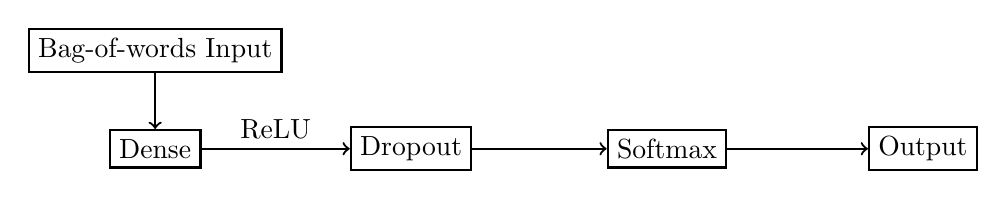
\begin{tikzpicture}[
            node distance=1.25cm,
            every node/.style={fill=white, font=\footnotesize},
            thick, scale=1, every node/.style={scale=1}]

        \node (input) [draw, align=center] {Bag-of-words Input};
        \node (dense) [draw, below of=input] {Dense};
        \draw[->] (input.south) -- (dense.north);
        \node (dropout) [draw, right of=dense, xshift=2cm] {Dropout};
        \draw[->] (dense.east) -- node[above, midway] {ReLU} (dropout.west);
        \node (softmax) [draw, right of=dropout, xshift=2cm] {Softmax};
        \draw[->] (dropout.east) -- (softmax.west);
        \node (output) [draw, right of=softmax, xshift=2cm] {Output};
        \draw[->] (softmax.east) -- (output.west);

    \end{tikzpicture}
    \caption{BoW + MLP architecture. The input article is encoded as a bag of words, then feed into a single linear multilayer perceptron before softmax operation.}
    \label{fig:bow_mlp_architecture}
\end{figure}

Figure \ref{fig:bow_mlp_architecture} shows the simple diagram of the BoW + MLP method, combining traditional encoding methods with a simple neural network training. This approach allows for a simple and computationally-cheap implementation, yet effective classifier. The model is trained on 10 epochs with a learning rate of 2e-5. Hidden size for the dense layer is 128 with a dropout probability of 0.2, no warmup steps are applied.

\subsection{BERT fine-tuning}

\begin{figure}[htbp]
    \centering
    \includegraphics[width=0.9\linewidth]{images/bert_finetuning.png}
    \caption{BERT pre-training and fine-tuning procedures \cite{devlin-2019-bert}}
    \label{fig:bert_finetuning}
\end{figure}

A fine-tuning operation is done as described in the original BERT paper \cite{devlin-2019-bert}, where input texts are tokenised and fed into a pre-trained BERT model for a downstream task. This approach leverages the powerful pre-trained representations from BERT and adapts them to the specific requirements of the downstream task with relatively small amounts of task-specific training data. This method has become a widely common and popular technique for performing various NLP tasks due to its effectiveness in improving performance over traditional models.

Fine-tuning is done over 4 epochs with weighted loss, 2e-5 learning rate, and 500 linear warmup steps.

\subsection{BERT sliding window fine-tuning}

\begin{figure}[htbp]
    \centering
    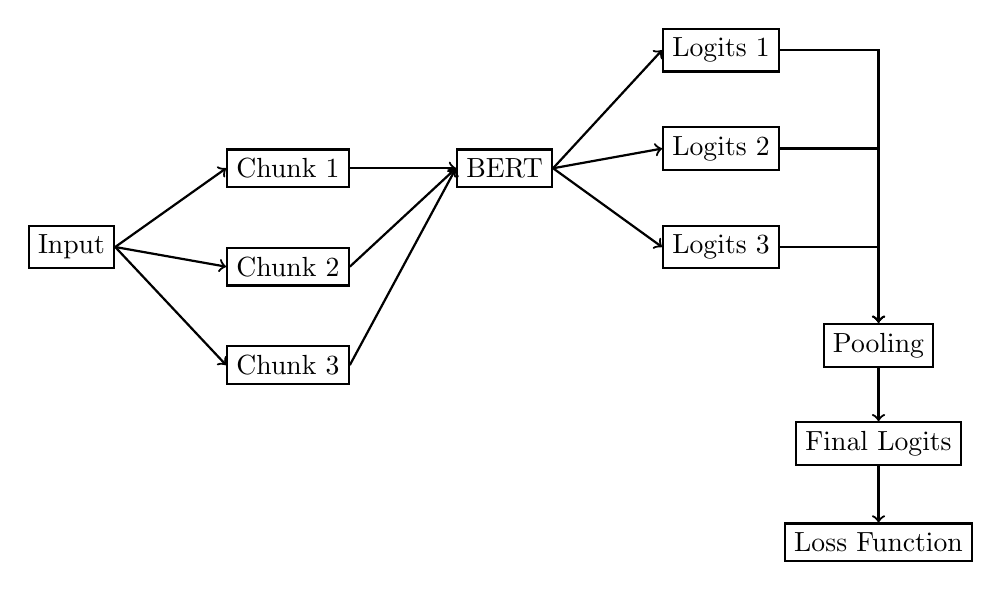
\begin{tikzpicture}[
            node distance=1.25cm,
            every node/.style={fill=white, font=\footnotesize},
            thick, scale=1, every node/.style={scale=1}
        ]

        \node (input) [draw, align=center] {Input};

        \node (chunk1) [draw, right of=input, xshift=1.5cm, yshift=1cm] {Chunk 1};
        \node (chunk2) [draw, below of=chunk1] {Chunk 2};
        \node (chunk3) [draw, below of=chunk2] {Chunk 3};

        \draw[->] (input.east) -- (chunk1.west);
        \draw[->] (input.east) -- (chunk2.west);
        \draw[->] (input.east) -- (chunk3.west);

        \node (bert) [draw, right of=chunk1, xshift=1.5cm] {BERT};

        \draw[->] (chunk1.east) -- (bert.west);
        \draw[->] (chunk2.east) -- (bert.west);
        \draw[->] (chunk3.east) -- (bert.west);

        \node (logits1) [draw, right of=bert, xshift=1.5cm, yshift=1.5cm] {Logits 1};
        \node (logits2) [draw, below of=logits1] {Logits 2};
        \node (logits3) [draw, below of=logits2] {Logits 3};

        \draw[->] (bert.east) -- (logits1.west);
        \draw[->] (bert.east) -- (logits2.west);
        \draw[->] (bert.east) -- (logits3.west);

        \node (pooling) [draw, below of=logits3, xshift=2cm, align=center] {Pooling};

        \draw[->] (logits1.east) -- ++(0.5cm,0) -| (pooling.north);
        \draw[->] (logits2.east) -- ++(0.5cm,0) -| (pooling.north);
        \draw[->] (logits3.east) -- ++(0.5cm,0) -| (pooling.north);

        \node (final_logits) [draw, below of=pooling] {Final Logits};

        \draw[->] (pooling.south) -- (final_logits.north);

        \node (loss) [draw, below of=final_logits] {Loss Function};

        \draw[->] (final_logits.south) -- (loss.north);
    \end{tikzpicture}
    \caption{BERT Sliding window fine-tuning architecture. The input article is split into chunks, each chunk is processed by the model as a mini batch, and the resulting logits are pooled before applying the loss function.}
    \label{fig:sliding_window_architecture}
\end{figure}

Figure \ref{fig:sliding_window_architecture} illustrates the architecture of the sliding window fine-tuning method. Input texts are segmented into chunks, which are then processed as mini-batches by the model. The logits (output scores) produced by each chunk are then pooled together to produce the final logits, to which the loss function is applied. This method bypasses the sequence length limitation of BERT models (512 tokens), allowing for full representation and processing of text input without any loss of information.

A window size of 512 is chosen in the implementation with no stride. Similarly, fine-tuning is done over 4 epochs with weighted loss, 2e-5 learning rate, and 500 linear warmup steps.

\begin{comment}
The complexity of this method is as follows:
\[
    O(L \cdot T \cdot H)
\]

where L is the sequence length, T is the number of Transformer layers in the BERT model (typically 12), H is Hidden size of the BERT model (dimension of the Transformer's feedforward networks, typically 768).
\end{comment}

\subsection{CLS method}


\begin{figure}[htbp]
    \centering

    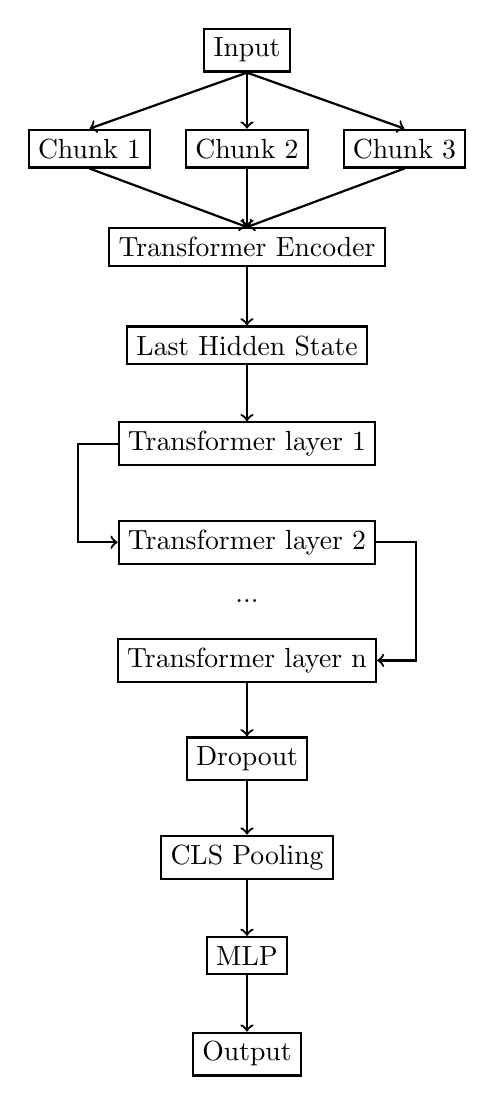
\begin{tikzpicture}[
            node distance=1.25cm,
            every node/.style={fill=white, font=\footnotesize},
            thick, scale=1, every node/.style={scale=1}]


        \node (input) [draw, align=center] {Input};

        \node (chunk1) [draw, below of=input, xshift=-2cm] {Chunk 1};
        \node (chunk2) [draw, below of=input] {Chunk 2};
        \node (chunk3) [draw, below of=input, xshift=2cm] {Chunk 3};

        \draw[->] (input.south) -- (chunk1.north);
        \draw[->] (input.south) -- (chunk2.north);
        \draw[->] (input.south) -- (chunk3.north);

        \node (encoder) [draw, below of=chunk2] {Transformer Encoder};

        \draw[->] (chunk1.south) -- (encoder.north);
        \draw[->] (chunk2.south) -- (encoder.north);
        \draw[->] (chunk3.south) -- (encoder.north);

        \node(hidden) [draw, below of=encoder] {Last Hidden State};

        \draw[->] (encoder.south) -- (hidden.north);

        \node (transformer1) [draw, below of=hidden] {Transformer layer 1};
        \node (transformer2) [draw, below of=transformer1] {Transformer layer 2};
        \node (transformern) [draw, below of=transformer2, yshift=-0.25cm] {Transformer layer n};
        \node (transformer_dots) [below of=transformer2, node distance=0.75cm] {...};

        \draw[->] (hidden.south) -- (transformer1.north);
        \draw[->] (transformer1.west) -- ++(-0.5cm,0) |- (transformer2.west);
        \draw[->] (transformer2.east) -- ++(0.5cm,0) |- (transformern.east);

        \node (dropout) [draw, below of=transformern] {Dropout};

        \draw[->] (transformern.south) -- (dropout.north);

        \node (cls) [draw, rectangle, below of=dropout] {CLS Pooling};

        \draw[->] (dropout.south) -- (cls.north);

        \node (mlp) [draw, rectangle, below of=cls] {MLP};

        \draw[->] (cls.south) -- (mlp.north);

        \node (output) [draw, rectangle, below of=mlp] {Output};

        \draw[->] (mlp.south) -- (output.north);


    \end{tikzpicture}
    \caption{CLS method architecture}
    \label{fig:cls_method}
\end{figure}

Figure \ref{fig:cls_method} shows the full architecture of the CLS method. This method begins by similarly segmenting the input text into smaller chunks. These chunks are encoded into a higher dimensional space features by feeding them into a pre-trained Large Language Model (LLM) and extracting the last hidden state, also known as \textit{feature-based approach} as described in \cite{sun-2020-fine-tune}. Subsequently, the encoded chunks are then passed into \textit{n}-amount of Transformer layers to enrich their contextual understanding. For each chunk afterwards, only the representation of the CLS token (the first token) is retained (CLS Pooling, as in \cite{su-2021-classifying}), serving as a concise summary of the entire chunk sequence. This summary representation is then processed through a Multi-Layer Perceptron (MLP). Lastly, a softmax operation will be applied to the output of the MLP layer to determine the final output class. Using a LLM as an encoder and taking its last hidden state allows for a good contextual representation of each chunk. By only using the CLS token representation instead of the whole chunk, this method allows for a more effective, yet simpler approach compared to other chunk pooling methods.

Two different language models can be used as the Transformer encoder in this method: BERT \cite{devlin-2019-bert} or MAGPIE \cite{horych-2024-magpie}. The MLP consists of two linear layers with ReLu activation function \cite{agarap-2018-relu} and dropouts. Each chunk is set to contain 512 tokens, only 2 Transformer layers are used, and 0.2 probability is applied to the dropout layer. Training is done over 3 epochs with weighted loss, 1e-5 learning rate and 162 warmup steps (10\% of total training steps).

\begin{comment}
The complexity of the CLS method can be expressed as:
\[
    O(L \cdot TF \cdot T \cdot H_{\text{enc}}^2 \cdot M \cdot H_{\text{mlp}}^2)
\]

where:
\begin{align*}
    L              & : \text{Sequence length (number of tokens)}, \\
    T              & : \text{Number of Transformer layers},       \\
    H_{\text{enc}} & : \text{Hidden size of Transformer layers},  \\
    M              & : \text{Number of layers in the MLP},        \\
    H_{\text{mlp}} & : \text{Hidden size of the MLP}.             \\
\end{align*}
\end{comment}

\section{Training details}

All methods are implemented in Python 3.12.0 \cite{van-1995-python} using the PyTorch \cite{paszke-2017-pytorch} and Transformer \cite{wolf-2020-huggingface} package from HuggingFace. The BERT model utilised in these methods is the 'bert-base-cased' instead of the 'bert-base-uncased' to account for distinctions in capitalised words, which may be crucial \cite{devlin-2019-bert}. AdamW \cite{loshchilov-2019-adamw} optimiser and Cross Entropy Loss is used in all cases. Batch size is set to 8 for all deep learning methods.

\subsection{Weighted loss}

Weighted loss addresses the problem of training models on an imbalanced dataset by assigning higher weights to classes with fewer instances and lower weights to classes with more instances. This adjustment ensures that the model pays more attention to correctly predicting the minority class, thereby improving overall performance metrics. Using weighted loss during training is preferred over oversampling the minority class. Oversampling can introduce abstract examples that may not accurately represent real-world articles, potentially leading to less effective model performance.

Weighted loss is calculated through the scikit-learn library \cite{pedregosa-2011-scikit-learn} and inserted into the loss function. Figure \ref{fig:class_weight} shows the calculated class weight for each class in the training set.


\begin{figure}[htbp]
    \centering
    \includegraphics[width=0.9\linewidth]{figures/class_weight.png}
    \caption{Class weight in the training set}
    \label{fig:class_weight}
\end{figure}



%%% Local Variables: 
%%% mode: latex
%%% TeX-master: "thesis"
%%% End: 

\chapter{Proposed Methods}
\label{cha:5}

\section{Features and baselines}

The main focus of the features will be the textual content of articles. A good article-level bias classifier should be able to generalise solely or mainly from the content of the articles, capturing context of the article will be the key element of a good performance.

As a baseline, traditional methods such as Bag-of-Words and TF-IDF along with standard fine-tuning of BERT are implemented.

\begin{comment}
Correlation between sentiment and bias?

Following from (\citealt{chen-2020-detecting-media-bias-gaussian},\citealt{van-den-berg-2020-contex-informational-bias-detection}, \citealt{guo-2022-modeling}, and \citealt{maab-2023-lexical-bias-detection}), experiments will be done with techniques from these past works, particularly on context-building.

Other representation techniques such as Doc2Vec \citep{mikolov-2014-doc2vec} and Multivec \citep{berard-2016-multivec} will also be considered.

Sentiment analysis can be beneficial as additional features, find relationships and correlation between sentiment and bias. (find ref)

MultiVec includes word2vec's features, paragraph vector (batch and online) and bivec for bilingual distributed representations. MultiVec also includes different distance measures between words and sequences of words.
\end{comment}

\begin{comment}
ChatGPT on article-level representations
Word Embeddings: Techniques like Word2Vec, GloVe, or FastText can convert words into numerical vectors, capturing semantic relationships between them. For an article representation, averaging or pooling these word vectors can create a simple yet effective representation.

Doc2Vec: Models like Doc2Vec extend word embeddings to whole documents, assigning each document a unique vector representation. This captures document-level semantics and context.

TF-IDF: Term Frequency-Inverse Document Frequency represents the importance of a word in a document relative to a collection of documents. It gives weight to words based on their frequency in the document and their rarity in the corpus.

BERT and Transformers: Models like BERT utilize transformer architectures to create contextualized word embeddings. By considering the context of words in a sentence, these models generate representations that capture nuanced meanings.

Graph-based Representations: Representing articles as nodes in a graph where edges signify relationships (such as co-citations or topic similarities) can offer a comprehensive representation.

Topic Modeling: Techniques like Latent Dirichlet Allocation (LDA) or Non-Negative Matrix Factorization (NMF) can help in extracting underlying topics from the articles, creating representations based on these topics' distributions.

P.S. from ChatGPT -> For very long documents, downsampling or breaking the article into manageable chunks might be necessary to fit into memory or improve model performance.
\end{comment}


\section{Evaluation}

\section{Proposed Method}

\section{Results}

%%% Local Variables: 
%%% mode: latex
%%% TeX-master: "thesis"
%%% End: 

\chapter{Evaluation}
\label{cha:6}

All methods are implemented using the PyTorch \cite{paszke-2017-pytorch} and transformer \cite{wolf-2020-huggingface} package from HuggingFace. The batch size is set to 8, with epochs ranging between 3-5. For every method, precision, recall, and F1 score is evaluated on both overall and per class performance. It is particularly important to assess how well the model classify biased articles.

\section{Baseline methods}

\begin{table}[htbp]
    \centering
    \begin{tabular}{|| c | c | c | c | c ||}
        \hline
        \multicolumn{5}{|| c ||}{\textbf{Features: title + content}} \\
        \hline
        Class              & Precision & Recall & F1     & Support   \\
        \hline
        Problematic        & 0.38      & 0.41   & 0.39   & 27        \\
        \hline
        Questionable       & 0.34      & 0.31   & 0.33   & 54        \\
        \hline
        Generally Reliable & 0.36      & 0.40   & 0.38   & 104       \\
        \hline
        Reliable           & 0.85      & 0.83   & 0.84   & 384       \\
        \hline
        Overall            & 0.6922    & 0.6818 & 0.6865 &           \\
        \hline
    \end{tabular}
    \caption{BoW + logistic regression evaluation}
    \label{table:bow-logistic-eval}
\end{table}

\begin{table}[htbp]
    \centering
    \begin{tabular}{|| c | c | c | c | c ||}
        \hline
        \multicolumn{5}{|| c ||}{\textbf{Features: title + content}} \\
        \hline
        Class              & Precision & Recall & F1     & Support   \\
        \hline
        Problematic        & 1.00      & 0.11   & 0.20   & 27        \\
        \hline
        Questionable       & 0.47      & 0.17   & 0.25   & 54        \\
        \hline
        Generally Reliable & 0.36      & 0.31   & 0.33   & 104       \\
        \hline
        Reliable           & 0.79      & 0.94   & 0.86   & 384       \\
        \hline
        Overall            & 0.6904    & 0.7117 & 0.6725 &           \\
        \hline
    \end{tabular}
    \caption{TF-IDF + logistic regression evaluation}
    \label{table:tfidf_logistic-eval}
\end{table}


In both Table \ref{table:bow-logistic-eval} and Table \ref{table:tfidf_logistic-eval}, it can be seen that frequency-based approaches such as BoW and TF-IDF perform generally well. Including outlet information as features only slighty improve the performance. However, when we look at per-class metrics, it can be seen that the overall scores are heavily influenced by the performance of class 'Reliable' due to its large support. Evidently, the model suffers when classifying underrepresented classes. Furthermore, TF-IDF model seems to perform significantly worse in the 'Problematic' class.

\begin{table}[htbp]
    \centering
    \begin{tabular}{|| c | c | c | c | c ||}
        \hline
        \multicolumn{5}{|| c ||}{\textbf{Features: title + content}}          \\
        \hline
        Class              & Precision & Recall & F1     & Support            \\
        \hline
        \hline
        Problematic        & 0.43      & 0.44   & 0.44   & 27                 \\
        \hline
        Questionable       & 0.29      & 0.39   & 0.33   & 54                 \\
        \hline
        Generally Reliable & 0.44      & 0.48   & 0.46   & 104                \\
        \hline
        Reliable           & 0.90      & 0.83   & 0.86   & 384                \\
        \hline
        Overall            & 0.7359    & 0.7065 & 0.7193 &                    \\
        \hline
        \hline
        \hline
        \hline
        \multicolumn{5}{|| c ||}{\textbf{Features: outlet + title + content}} \\
        \hline
        Class              & Precision & Recall & F1     & Support            \\
        \hline
        \hline
        Problematic        & 0.65      & 0.56   & 0.60   & 27                 \\
        \hline
        Questionable       & 0.45      & 0.50   & 0.47   & 54                 \\
        \hline
        Generally Reliable & 0.44      & 0.62   & 0.52   & 104                \\
        \hline
        Reliable           & 0.94      & 0.84   & 0.88   & 384                \\
        \hline
        Overall            & 0.8186    & 0.7883 & 0.7504 &                    \\
        \hline
    \end{tabular}
    \caption{BERT fine-tuning evaluation}
    \label{table:bert-fine-tuning-eval}
\end{table}

Fine-tuning BERT after 6 epochs only performed slightly better than BoW method as can be seen in Table \ref{table:bert-fine-tuning-eval} and Table \ref{table:bow-logistic-eval}. In this method 'bert-base-cased' is used instead of 'bert-base-uncased' to reserve differences in capitalised words, which can be crucial. Moreover, incorporating outlet information as features moderately increase the performance in all accounts.

\begin{table}[htbp]
    \centering
    \begin{tabular}{|| c | c | c | c | c ||}
        \hline
        Class              & Precision & Recall & F1     & Support \\
        \hline
        \hline
        Problematic        & 0.56      & 0.70   & 0.62   & 27      \\
        \hline
        Questionable       & 0.58      & 0.46   & 0.52   & 54      \\
        \hline
        Generally Reliable & 0.56      & 0.53   & 0.54   & 104     \\
        \hline
        Reliable           & 0.91      & 0.93   & 0.92   & 384     \\
        \hline
        Overall            & 0.7945    & 0.7996 & 0.7959 &         \\
        \hline
    \end{tabular}
    \caption{Outlet-based majority votes evaluation}
    \label{table:majority-votes-eval}
\end{table}



As a comparison, using solely outlet information without any textual information (with majority votes) outperformed all baseline methods both overall and in every class. This result signifies how influential outlet information can be used to classify media bias.

\begin{comment}
Find out why TF-IDF performs worse on class problematic
\end{comment}


\section{Sliding window}

For this approach, a window size of 512 (maximum token of BERT) is chosen with a stride of 256. Additionally, only the first 3 chunks of each input sequence will be used and the rest discarded, as using longer chunks did not consistently improve performance, along with increased computation cost.


\begin{table}[htbp]
    \centering
    \begin{tabular}{|| c | c | c | c | c ||}
        \hline
        \multicolumn{5}{|| c ||}{\textbf{Features: title + content}}          \\
        \hline
        Class              & Precision & Recall & F1     & Support            \\
        \hline
        \hline
        Problematic        & 0.45      & 0.48   & 0.46   & 27                 \\
        \hline
        Questionable       & 0.39      & 0.52   & 0.45   & 54                 \\
        \hline
        Generally Reliable & 0.42      & 0.50   & 0.46   & 104                \\
        \hline
        Reliable           & 0.91      & 0.81   & 0.86   & 384                \\
        \hline
        Overall            & 0.7472    & 0.7112 & 0.7257 &                    \\
        \hline
        \hline
        \hline
        \hline
        \multicolumn{5}{|| c ||}{\textbf{Features: outlet + title + content}} \\
        \hline
        Class              & Precision & Recall & F1     & Support            \\
        \hline
        \hline
        Problematic        & 0.46      & 0.41   & 0.43   & 27                 \\
        \hline
        Questionable       & 0.41      & 0.48   & 0.44   & 54                 \\
        \hline
        Generally Reliable & 0.46      & 0.56   & 0.51   & 104                \\
        \hline
        Reliable           & 0.91      & 0.84   & 0.87   & 384                \\
        \hline
        Overall            & 0.7585    & 0.7359 & 0.7451 &                    \\
        \hline
    \end{tabular}
    \caption{Sliding Window evaluation}
    \label{table:sliding-window-eval}
\end{table}

The sliding window method outperformed both BoW and TF-IDF methods, while performing slightly better to a standard BERT fine-tuning of the first 512 tokens. However, with the outlet information included, BERT fine-tuning still reigns superior with a particularly strong f1 score on the "Problematic" class.

\section{CLS Method}

For the CLS method, two different language models are used: BERT and MAGPIE, to encode the input in a higher dimensional space. Both approaches with the CLS method are evaluated. A chunk size of 512 is used, 2 transformer layers, learning rate 1e-5, 162 warmup steps (10\% of training steps), 0.2 dropout probability, and 3 epochs.


\begin{table}[htbp]
    \centering
    \begin{tabular}{|| c | c | c | c | c ||}
        \hline
        \multicolumn{5}{|| c ||}{\textbf{Features: title + content}}          \\
        \hline
        Class              & Precision & Recall & F1     & Support            \\
        \hline
        \hline
        Problematic        & 0.44      & 0.67   & 0.53   & 27                 \\
        \hline
        Questionable       & 0.41      & 0.48   & 0.44   & 54                 \\
        \hline
        Generally Reliable & 0.39      & 0.50   & 0.44   & 104                \\
        \hline
        Reliable           & 0.91      & 0.79   & 0.84   & 384                \\
        \hline
        Overall            & 0.7440    & 0.6994 & 0.7163 &                    \\
        \hline
        \hline
        \hline
        \hline
        \multicolumn{5}{|| c ||}{\textbf{Features: outlet + title + content}} \\
        \hline
        Class              & Precision & Recall & F1     & Support            \\
        \hline
        \hline
        Problematic        & 0.37      & 0.59   & 0.46   & 27                 \\
        \hline
        Questionable       & 0.32      & 0.43   & 0.37   & 54                 \\
        \hline
        Generally Reliable & 0.40      & 0.47   & 0.43   & 104                \\
        \hline
        Reliable           & 0.92      & 0.79   & 0.85   & 384                \\
        \hline
        Overall            & 0.7384    & 0.6871 & 0.7071 &                    \\
        \hline
    \end{tabular}
    \caption{BERT CLS evaluation}
    \label{table:bert-cls-eval}
\end{table}


\begin{table}[htbp]
    \centering
    \begin{tabular}{|| c | c | c | c | c ||}
        \hline
        \multicolumn{5}{|| c ||}{\textbf{Features: title + content}}          \\
        \hline
        Class              & Precision & Recall & F1     & Support            \\
        \hline
        \hline
        Problematic        & 0.46      & 0.63   & 0.53   & 27                 \\
        \hline
        Questionable       & 0.36      & 0.41   & 0.38   & 54                 \\
        \hline
        Generally Reliable & 0.41      & 0.55   & 0.47   & 104                \\
        \hline
        Reliable           & 0.93      & 0.80   & 0.86   & 384                \\
        \hline
        Overall            & 0.7577    & 0.7117 & 0.7293 &                    \\
        \hline
        \hline
        \hline
        \hline
        \multicolumn{5}{|| c ||}{\textbf{Features: outlet + title + content}} \\
        \hline
        Class              & Precision & Recall & F1     & Support            \\
        \hline
        \hline
        Problematic        & 0.42      & 0.52   & 0.47   & 27                 \\
        \hline
        Questionable       & 0.35      & 0.43   & 0.38   & 54                 \\
        \hline
        Generally Reliable & 0.43      & 0.55   & 0.48   & 104                \\
        \hline
        Reliable           & 0.93      & 0.82   & 0.87   & 384                \\
        \hline
        Overall            & 0.76034   & 0.7170 & 0.7342 &                    \\
        \hline
    \end{tabular}
    \caption{MAGPIE CLS evaluation}
    \label{table:magpie-cls-eval}
\end{table}

Similarly, both CLS methods mostly outperformed the baselines. However, with outlet information included the CLS methods performed somewhat worse, particularly on the most biased "Problematic" class.

%%% Local Variables: 
%%% mode: latex
%%% TeX-master: "thesis"
%%% End: 

\chapter{Conclusion}
\label{cha:7}

Simple, frequency-based methods such as BoW and TF-IDF combined with logistic regression already provided decent result given the circumstances.

While we can seemingly just take the outlet and use this information to classify media bias...

Furthermore, we have not tested the model with unseen data containing unseen outlets...

\subsection{Future Work}

The methods need to be reevaluated with a bigger dataset and particularly much more examples of biased articles, as the current dataset is highly-imbalanced.

Classifying media bias right now, in this way, does not provide much explanaibility. Ultimately, we would want a model to also output a reasoning behind the classification.

Implement a more global methods using graph-based approach to encode multiple articles and define relationships between them.

Carefully tune the test set to enable more representational metric, include unseen outlets.

%%% Local Variables: 
%%% mode: latex
%%% TeX-master: "thesis"
%%% End: 


% If you have appendices:
\appendixpage*          % if wanted
\appendix
\chapter{The First Appendix}
\label{app:A}

\begin{figure}[htbp]
    \centering
    \includegraphics[width=0.9\linewidth]{figures/tokens_count_vx_split_hist.png}
    \caption{Articles tokens count distribution}
    \label{fig:tokens_hist_split}
\end{figure}

\begin{figure}[htbp]
    \centering
    \includegraphics[width=0.7\linewidth]{figures/wordcloud_vx.png}
    \caption{Wordcloud}
    \label{fig:wordcloud}
\end{figure}


\begin{figure}[htbp]
    \centering
    \includegraphics[width=0.8\linewidth]{figures/tokens_count_vx_per_class_hist.png}
    \caption{Average tokens count per class}
    \label{fig:avg_tokens_count_per_class}
\end{figure}


\begin{figure}[htbp]
    \centering
    \includegraphics[width=0.8\linewidth]{images/Media-Bias-Chart-12.0_Jan-2024-Licensed-scaled.jpg}
    \caption{Ad Fontes media bias chart}
    \label{fig:adfontes-media-bias-chart}
\end{figure}

\begin{figure}[htbp]
    \centering
    \includegraphics[width=0.9\linewidth]{images/statistic_id657090_ability-to-recognize-false-information-and-news-in-the-us-2023.png}
    \caption{Ability to recognise false information in the US \cite{yougov-2023-confidence}}
    \label{fig:ability-to-recognize-false-information-and-news-in-the-us-2023}
\end{figure}

\begin{figure}[htbp]
    \centering
    \includegraphics[width=0.6\linewidth]{images/statistic_id308468_trustworthiness-of-news-media-worldwide-2023.png}
    \caption{Trustworthiness of news media worldwide, as of February 2023 \cite{reuters-2023-trust}}
    \label{fig:trustworthiness-of-news-media-worldwide-2023}
\end{figure}



%%% Local Variables: 
%%% mode: latex
%%% TeX-master: "thesis"
%%% End: 

% ... and so on until
% \chapter{The Last Appendix}
\label{app:n}

%%% Local Variables: 
%%% mode: latex
%%% TeX-master: "thesis"
%%% End: 


\backmatter
% The bibliography comes after the appendices.
% You can replace the standard "abbrv" bibliography style by another one.
\bibliographystyle{abbrv}
\bibliography{references}

\end{document}

%%% Local Variables: 
%%% mode: latex
%%% TeX-master: t
%%% End: 
